\documentclass[12pt]{article}
\usepackage{preamble}

\pagestyle{fancy}
\fancyhead[LO,LE]{Математический анализ}
\fancyhead[CO,CE]{07.02.2024}
\fancyhead[RO,RE]{Лекции Далевской О. П.}


\begin{document}
    \section{1. Определенный интеграл}


    \section{1.1. Задача и определение}

    \underline{Задача}. Дана криволинейная фигура:


    \begin{center}
        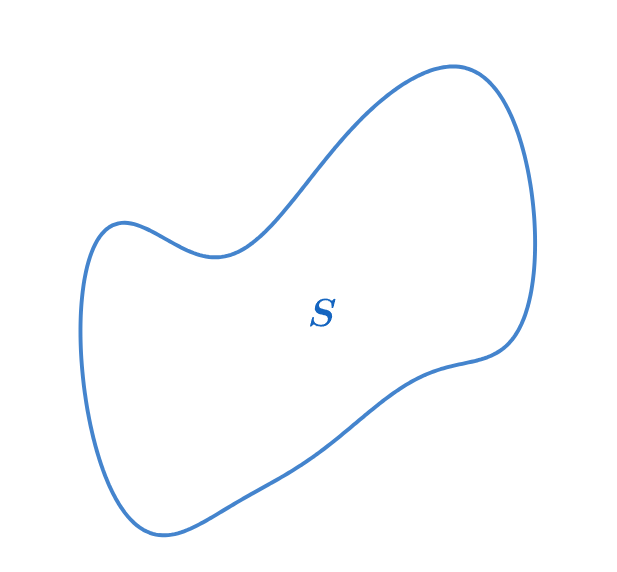
\includegraphics[height=7cm]{images/calculus_2024_02_07_0}
    \end{center}

    Надо найти ее площадь S

    Произведем ее дробление на маленькие элементарные фигуры, площадь которых мы можем посчитать:

    \begin{center}
        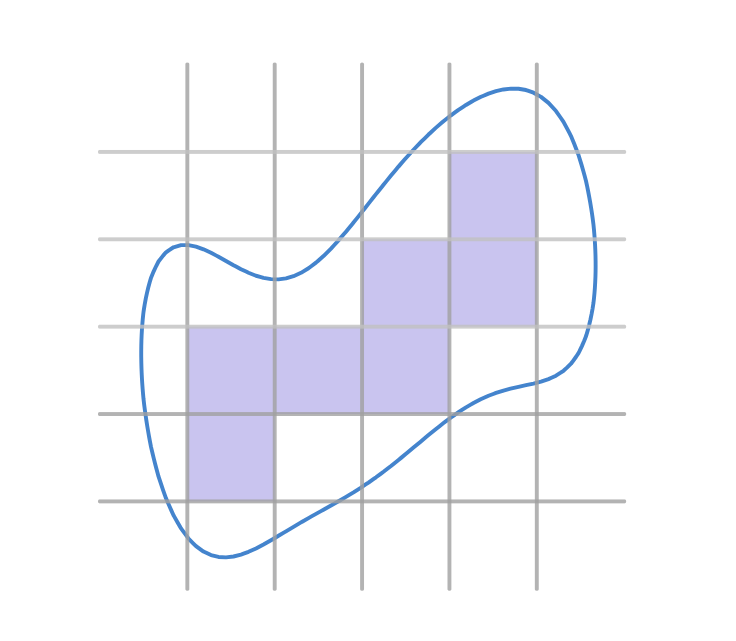
\includegraphics[height=7cm]{images/calculus_2024_02_07_1}
    \end{center}

    Уменьшаем дробление, чтобы свести погрешность к 0 (погрешность между истинной площадью и суммарной площадью прямоугольников)

    Сведем задачу к простейшей в ДПСК:

    \vspace{10mm}


    \begin{multicols}{2}
        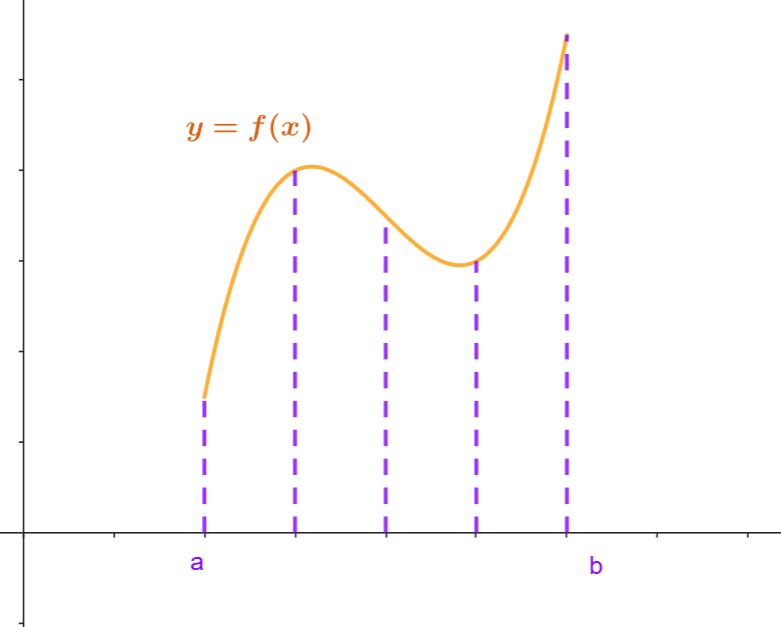
\includegraphics[height=6cm]{images/calculus_2024_02_07_2}

        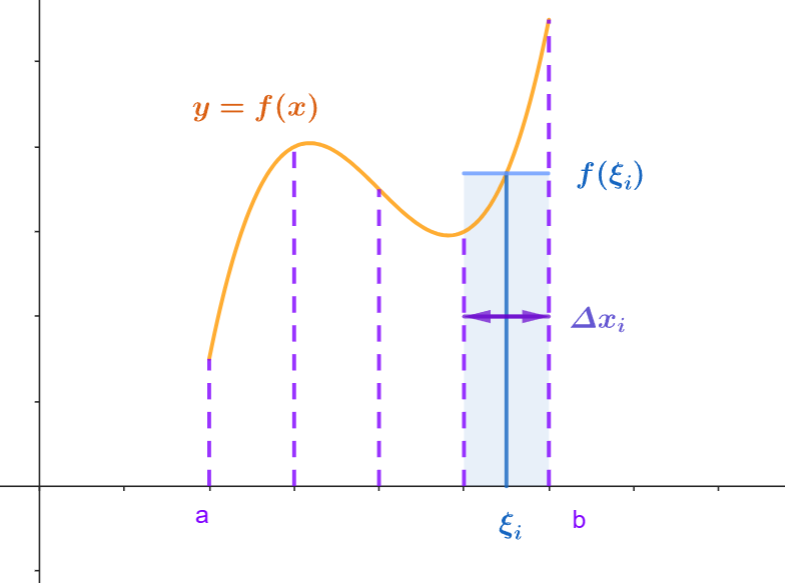
\includegraphics[height=6cm]{images/calculus_2024_02_07_3}
    \end{multicols}

    \begin{enumerate}
        \item Вводим разбиение отрезка $[a; b]\ (a < b)$ точками $\displaystyle a < x_0 < \dots < x_n < b$

        $\displaystyle T = \Set{x_i}^n_{i=0}$

        \item Выбираем средние точки на частичных отрезках $\displaystyle [x_{i-1}, x_i]^n_{i=1}$

        $\displaystyle \Set{\xi_i}_{i=1}^n$ - набор средних точек

        $\displaystyle \Delta x_i \stackrel{\text{обозн.}}{=} x_i - x_{i-1}$ - длина отрезка

        \item Строим элементарные прямоугольники
        \item Составляем сумму площадей всех таких прямоугольников:

        \[\sigma_n = \sum^n_{i=1} \Delta x_i f(\xi_i)\]

        - интегральная сумма Римана

        \item Заменяя разбиение, выбор $\displaystyle \xi_i$ при каждом $n$, получаем последовательность $\displaystyle \Set{\sigma_n}$

        При этом следим, чтобы ранг разбиения $\displaystyle \tau = \max\limits_{1 \leq i \leq n} \Delta x_i \rightarrow 0$ при $n \to \infty$

        Иначе получим неуничтожаемую погрешность

        \item \Def Если существует конечный предел интегральной суммы и он не зависит от типа,
        ранга дробления и выбора средних точек, то он называется определенным интегралом

        \[\lim_{n\to\infty,\ \tau\to0} \sigma_n = \lim_{n\to\infty,\ \tau\to0} \sum^n_{i=1} \Delta x_i f(\xi_i) \stackrel{\text{def}}{=} \int_a^b f(x)dx\]

    \end{enumerate}

    \Nota Независимость от дробления и выбора средних точек существенна

    \Ex $\mathcal{D} = \begin{cases}
                           1,\ x \in [0, 1], x \not\in \mathbb{Q} \\ 0,\ x \in [0, 1], x \in \mathbb{Q}
    \end{cases}$

    Сумма Римана для этой функции неопределенна, так как все зависит от выбора средних точек:
    \begin{itemize}
        \item если средние точки иррациональные, то сумма равна единице
        \item иначе сумма равна нулю
    \end{itemize}

    В обозначении определенного интеграла $a$ и $b$ называют нижним и верхним пределами интегрирования соответственно

    Дифференциал $dx$ имеет смысл $\Delta x$, понимается как б. м., то есть:

    $f(x) dx$ - площадь элементарных прямоугольников, тогда

    $\displaystyle \int^b_a f(x) dx$ - сумма этих прямоугольников

    \vspace{5mm}

    \begin{enumerate}
        \item $\displaystyle \int_a^a f(x)dx \stackrel{\text{def}}{=} 0$
        \item $\displaystyle \int_a^b f(x)dx = -\int_b^a f(x)dx$
    \end{enumerate}

    Можно доказать, что определенный интеграл существует для всякой непрерывной на отрезке функции

    \underline{Геом. смысл}. Заметим в определении площадь подграфика функции $(f(x) \geq 0)$

    Заметим, что для $\displaystyle f(x) \leq 0 \quad \int_a^b f(x)dx = -S$


    \section{1.2. Свойства}

    \begin{enumerate}
        \item Линейность пределов $\Longrightarrow$ линейность пределов

        $\displaystyle \lambda \int^b_a f(x)dx + \mu \int^b_a g(x)dx = \int^b_a (\lambda f(x) + \mu g(x)) dx \quad (\lambda, \mu \in \Real)$

        \item Аддитивность (часто для кусочно-непрерывных функций с конечным числом точек разбивается на участки непрерывности)

        $\displaystyle \int^b_a f(x)dx + \int^c_b f(x)dx = \int^c_a f(x)dx$

        Доказательства строятся на свойствах конечных сумм и пределов

        \item Оценка определенного интеграла

        $f(x)$ непрерывна на $[a; b]$ (имеет наимен. ($m$) и наибол. ($M$) значения). Тогда:

        $\displaystyle m (b-a) \leq \int^b_a f(x)dx \leq M(b - a)$

        $\Box$ Док-во:

        По теореме Вейерштрасса 2 $f(x)$ принимает наименьшее и наибольшее значения и для всякого $x$ из $[a; b]$:  $m <= f(x) <= M$

        Так как все средние точки принадлежат $[a; b]$, то

        $\displaystyle m \leq f(\xi_i) \leq M \quad \forall \xi_i$

        $\displaystyle m \Delta_i \leq f(\xi_i) \Delta_i \leq M \Delta_i$

        $\displaystyle m \sum_{i=1}^n \Delta x_i \leq f(\xi_i) \sum_{i=1}^n \Delta x_i \leq M \sum_{i=1}^n \Delta x_i$

        Предельный переход:

        $\displaystyle \lim_{n\to\infty,\ \tau\to0} m \sum_{i=1}^n \Delta x_i \leq \int^b_a f(x) dx \leq \lim_{n\to\infty,\ \tau\to0} M \sum_{i=1}^n \Delta x_i$

        $\displaystyle m \lim_{n\to\infty,\ \tau\to0} \sum_{i=1}^n \Delta x_i \leq \int^b_a f(x) dx \leq M \lim_{n\to\infty,\ \tau\to0} \sum_{i=1}^n \Delta x_i$

        $\displaystyle m (b - a) \leq \int^b_a f(x) dx \leq M (b - a)$

        $\Box$


        \item \Th Лагранжа о среднем (в интегральной форме)

        $\displaystyle f(x) \in C^\prime_{[a,b]} \Longrightarrow \exists \xi \in (a, b) \ f^\prime(\xi) = \frac{f(b) - f(a)}{b - a}$

        Тогда найдется такая средняя точка, что

        $\displaystyle f(x) \in C_{[a,b]} \Longrightarrow \exists \xi \in (a, b) \ f(\xi)(b - a) = \int^b_a f(x)dx$

        % help me

        $\Box$

        $\displaystyle m \leq \underset{\text{некоторое число}}{\undergroup{\frac{1}{b-a} \int_a^b f(x)dx}} \leq M$ по свойству выше

        По теореме Больцано-Коши $f(x)$ непрерывна, поэтому пробегает все значения от $m$ до $M$

        Значит найдется такая точка $\xi$, что $\displaystyle f(\xi) = \frac{1}{b-a} \int_a^b f(x)dx$

        $\Box$

        \item Сравнение интегралов

        $\displaystyle f(x), g(x) \in C_{[a, b]} \quad \forall x \in [a, b] \quad f(x) \geq g(x)$

        Тогда $\displaystyle \int_a^b f(x)dx \geq \int_a^b g(x)dx$

        $\Box$

        $\displaystyle \int_a^b f(x)dx - \int_a^b g(x)dx = \int_a^b (f(x) - g(x))dx =
        \lim_{n\to\infty,\ \tau\to0} \sum_{i=1}^n \underset{\geq 0}{\undergroup{(f(\xi_i) - g(\xi_i))}} \underset{\geq 0}{\undergroup{\Delta x_i}} \geq 0$

        $\Box$


        \item Интеграл и модуль

        $\displaystyle \left| \int^b_a f(x)dx \right| \leq \int^b_a |f(x)| dx$

        $\Box$

        $\displaystyle \int^b_a f(x)dx = \lim_{n\to\infty,\ \tau\to0} \sum_{i=1}^n f(\xi_i) \Delta x_i = \lim_{n\to\infty} \sigma_n$

        $\displaystyle \int^b_a |f(x)|dx = \lim_{n\to\infty,\ \tau\to0} \sum_{i=1}^n |f(\xi_i)| \Delta x_i$

        Докажем, что $\displaystyle \lim_{n\to\infty} |\sigma_n| = |\lim_{n\to\infty} \sigma_n|$

        Так как определен $\displaystyle \int^b_a f(x)dx = \lim_{n\to\infty} \sigma_n = S \in \Real$, то можно рассмотреть случаи

        $\displaystyle S > 0: \quad \exists n_0 \ \forall n > n_0 \ \sigma_n > 0$ (вблизи $S$)

        $\displaystyle \lim_{n\to\infty} |\sigma_n| = |\lim_{n\to\infty} \sigma_n|$

        $\displaystyle S > 0: \quad \exists n_0 \ \forall n > n_0 \ \sigma_n < 0$ (вблизи $S$)

        $\displaystyle \lim_{n\to\infty} |\sigma_n| = -\lim_{n\to\infty} \sigma_n = |\lim_{n\to\infty} \sigma_n|$

        $\displaystyle S = 0: \lim_{n\to\infty} |\sigma_n| = |\lim_{n\to\infty} \sigma_n| = 0$

        $\displaystyle \left| \int^b_a f(x)dx \left| = |\lim_{n\to\infty} \sigma_n| = \lim_{n\to\infty} |\sigma_n| =
        \lim_{n\to\infty,\ \tau\to0} \left|\sum_{i=1}^n f(\xi_i) \Delta x_i\right| \leq \lim_{n\to\infty,\ \tau\to0} \sum_{i=1}^n |f(\xi_i)| \Delta x_i$ (модуль суммы меньше или равен сумме модулей)

        $\Box$

    \end{enumerate}

    \Nota Интеграл и разрыв

    Изъятие из отрезка не более, чем счетного числа точек, не меняет значение интеграла, что позволяет считать интеграл на интервале

    \Nota Сходимость интеграла - в определении интеграла подчеркивается, что это число.
    Если предел интегральных сумм не существует или бесконечен, говорят, что интеграл расходится

    \Nota Вычисления

    Определение дает способ вычисления и его можно упростить:

    $\displaystyle \forall i\ \Delta x_i = \Delta x, \quad \xi_i = \begin{sqcases}x_{i-1} \\ x_i\end{sqcases}$ - концы отрезка

    Так вычисляют \enquote{неберущиеся интегралы}

    Для функций, у которых первообразные выражаются в элементарных функциях используется не этот метод, а формула Ньютона-Лейбница

    \section{1.3. Вычисление определенного интеграла}



\end{document}
